\documentclass[11pt,letter,]{article}
\usepackage[]{mathpazo}
\usepackage{setspace}
\setstretch{1.5}
\usepackage{amssymb,amsmath}
\usepackage{ifxetex,ifluatex}
\usepackage{fixltx2e} % provides \textsubscript
\ifnum 0\ifxetex 1\fi\ifluatex 1\fi=0 % if pdftex
  \usepackage[T1]{fontenc}
  \usepackage[utf8]{inputenc}
\else % if luatex or xelatex
  \ifxetex
    \usepackage{mathspec}
  \else
    \usepackage{fontspec}
  \fi
  \defaultfontfeatures{Ligatures=TeX,Scale=MatchLowercase}
  \newcommand{\euro}{€}
\fi
% use upquote if available, for straight quotes in verbatim environments
\IfFileExists{upquote.sty}{\usepackage{upquote}}{}
% use microtype if available
\IfFileExists{microtype.sty}{%
\usepackage{microtype}
\UseMicrotypeSet[protrusion]{basicmath} % disable protrusion for tt fonts
}{}
\usepackage[margin=1.2in]{geometry}
\usepackage{hyperref}
\PassOptionsToPackage{usenames,dvipsnames}{color} % color is loaded by hyperref
\hypersetup{unicode=true,
            pdftitle={Effects of growth and recruitment assumptions in the status and management advice of the Chilean yellow lobster squat, Cervimunida johni},
            pdfauthor={Mariella Canales, Juan-Carlos Quiroz, Rodrigo Wiff, et al.},
            pdfsubject={aaaaa},
            colorlinks=true,
            linkcolor=blue,
            citecolor=blue,
            urlcolor=blue,
            breaklinks=true}
\urlstyle{same}  % don't use monospace font for urls
\usepackage{graphicx,grffile}
\makeatletter
\def\maxwidth{\ifdim\Gin@nat@width>\linewidth\linewidth\else\Gin@nat@width\fi}
\def\maxheight{\ifdim\Gin@nat@height>\textheight\textheight\else\Gin@nat@height\fi}
\makeatother
% Scale images if necessary, so that they will not overflow the page
% margins by default, and it is still possible to overwrite the defaults
% using explicit options in \includegraphics[width, height, ...]{}
\setkeys{Gin}{width=\maxwidth,height=\maxheight,keepaspectratio}
\setlength{\emergencystretch}{3em}  % prevent overfull lines
\providecommand{\tightlist}{%
  \setlength{\itemsep}{0pt}\setlength{\parskip}{0pt}}
\setcounter{secnumdepth}{5}

%%% Use protect on footnotes to avoid problems with footnotes in titles
\let\rmarkdownfootnote\footnote%
\def\footnote{\protect\rmarkdownfootnote}

%%% Change title format to be more compact
\usepackage{titling}

% Create subtitle command for use in maketitle
\newcommand{\subtitle}[1]{
  \posttitle{
    \begin{center}\large#1\end{center}
    }
}

\setlength{\droptitle}{-2em}
  \title{Effects of growth and recruitment assumptions in the status and
management advice of the Chilean yellow lobster squat, \emph{Cervimunida
johni}}
  \pretitle{\vspace{\droptitle}\centering\huge}
  \posttitle{\par}
\subtitle{aaaaa}
  \author{Mariella Canales, Juan-Carlos Quiroz, Rodrigo Wiff, et al.}
  \preauthor{\centering\large\emph}
  \postauthor{\par}
  \predate{\centering\large\emph}
  \postdate{\par}
  \date{May, 2016}



%\usepackage[switch*,modulo,running]{lineno}
\usepackage[running]{lineno}

\usepackage{fancyhdr}
% \pagestyle{fancy}
\fancyhf{}
% \fancyhead[LE,RO]{}
% \fancyhead[RE,LO]{\textit{draft 0.01}}
% \fancyfoot[RE,LO]{\leftmark}
% \fancyfoot[LE,RO]{\thepage}

\lhead[\rm\thepage]{\fancyplain{}{\sl{\itshape\nouppercase{\leftmark}}}}
\rhead[\fancyplain{}{\sl{\itshape\nouppercase{\leftmark}}}]{\rm\thepage}
\chead{}\lfoot{}\rfoot{\textit{draft 0.01}}\cfoot{}
\pagestyle{fancy}

\renewcommand{\headrulewidth}{0.3pt}
\renewcommand{\footrulewidth}{0.3pt}

\linenumbers

\setlength{\parindent}{25pt}
\setlength{\parskip}{0em}

\usepackage[table,xcdraw]{xcolor}

% Redefines (sub)paragraphs to behave more like sections
\ifx\paragraph\undefined\else
\let\oldparagraph\paragraph
\renewcommand{\paragraph}[1]{\oldparagraph{#1}\mbox{}}
\fi
\ifx\subparagraph\undefined\else
\let\oldsubparagraph\subparagraph
\renewcommand{\subparagraph}[1]{\oldsubparagraph{#1}\mbox{}}
\fi

\begin{document}
\maketitle
\begin{abstract}
This is the abstract.

It consists of two paragraphs.
\end{abstract}

\section{Introduction}\label{introduction}

The crustacean fisheries off central south Chile date back to 1953 when
the species yellow squat lobster (\emph{Cervimunida johni}) and red
squat lobster (\emph{Pleuroncodes monodon}) began to be exploited. Since
1972 landings of both species started to differentiate and the maximum
landings (10.322 tones) of yellow squat lobster was registered in 1997
(Canales and Arana 2012). The yellow squat lobster was divided in two
fisheries units in 1996 that nowadays correspond to 26º03'LS - 30º30'LS
(North Unit) and 30º30'LS -38º48'LS (South Unit) (Canales and Arana
2012; Bucarey 2015). This work is developed for the North fishery unit
of the Chilean yellow squat lobster.

The current fishery management of the squat lobster fisheries in Chile
is based on the total allowed catch (TAC) system. Decisions about catch
level are based on the status of the squat lobsters referred to the
current level of spawning biomass that allow the stock to be near or
around the maximum sustainable yield (MSY) (Bucarey et al. 2015). To
estimate the spawning biomass a single-species stock assessment model is
used. The model corresponds to an integrated age-structure model
(Maunder and Punt 2013) that encompasses multiple data types to reveal
the population dynamics and estimate both model parameters and derived
population and management outputs. However, because in crustacean
species age assignation is difficult, length composition data is used to
fit the model.

Maunder and Piner (2015) discussed that critical biological and
fisheries processes such as growth, natural mortality, recruitment, and
selectivity are still issues that remain unsolved in stock assessment
models, and without this knowledge, assumptions need to be made. However
incorrect assumptions can have a substantial impact on stock assessment
results and management advice. For instance, (Aires-da-Silva \emph{et
al.} 2015) showed that the estimated depletion level (ratio of the
spawning biomass) and fishing mortality rates were highly sensitive to
the assumed value of \(L_{\infty}\) as well as the variability of
length-at-age.

In the Chilean yellow squat lobster stock assessment model, two
important population process, individual growth and recruitment, carried
important assumptions. The mean length-at age in the growth process
follows the von Bertalanffy function with parameters \(k\) and
\(L_{\infty}\) assumed fixed and obtained from external studies. The
mean length at the first age (L1) as well as the coefficient of
variation of the mean length at age (VLA) are estimated in the model in
order to fit the length composition data that is converted to age
through a simulated length-at-age key. The recruitment process is
modelled with underlying the assumption that a Beverton and Holt (BH)
stock-recruitment relationship exist with a steepness value of \(h=1\).
The assumption is based in the lack of reliability of the Chilean yellow
squat lobster data to estimate the BH stock recruitment relationship
(Paya et al. 2014). Thus, the recruitment is modelled through annual
random deviations that follows a lognormal distribution with a variance
that is assumed fixed, while the averaged recruitment and annual
deviations are parameters to be estimated. Here, we aim to investigate
the impact of the assumptions of growth and recruitment process in the
stock assessment results and management advice indicators of the Chilean
yellow squat lobster fishery. We used the stock assessment models
developed for the Chilean squat lobster fisheries (Bucarey et al. 2015)
to carry a sensitivity analysis of different scenarios of the L1 and
VLA, in combination with scenarios of h and the coefficient of variation
of the recruitment (CVR). The response of five variables of the stock
assessment results were analyzed as well as five used for management
advice. Later, a simulation analysis was conducted to assess the
precision of the stock assessment model in estimates the parameters that
cause the higher variation in the stock assessment results and
management advice variables.

\section{Methods}\label{methods}

\subsection{Yellow squat lobster stock assessment
model}\label{yellow-squat-lobster-stock-assessment-model}

The Chilean yellow squat lobster model assume that in the north part
(26°03'-30°30' LS) of the distribution area of the species there is a
closed stock of yellow squat lobster independently of south stock. The
assessment covers a period of time from 1985 to 2015 and encompasses the
following sources of data, i) official landings, ii) catch per unit
effort (CPUE), iii) survey biomass and iv) length composition of the
catches and survey. Biological parameters such us, natural mortality,
maturity and growth are estimated outside the model. Growth is
differentiated by sex, natural mortality is invariant and the
vulnerability to the fishing gear and survey is invariant and follows a
logistic function. The observation model of the landings, CPUE, and
biomass survey assume a lognormal distribution of the error and the
length composition of the catches and survey assume a multinomial
distribution. The parameters are estimated by the minimization of the
sum of the negative log-likelihood of each time series. The yellow squat
lobster model is implemented in a computational routine in the software
AD Model Builder for non-lineal statistical models
(\url{http://admb-project.org/}). Although the stock assessment model of
the yellow squat lobster is available at \url{http://www.ifop.cl}. we
present in the Appendix section a summary of the mathematical
description of the stock assessment model.

\subsection{Performance measures}\label{performance-measures}

To measures the impact of the effect of the assumptions of growth and
recruitment in the stock assessment result and management advice
indicators the following variable were used. Total biomass in the last
year (TB), spawning biomass in the last year (SB), averaged recruitment
(R), yield at the target referent point (\(Y_{MSY}\)), virginal spawning
biomass (BD\(_0\)). We also analyzed the effect in the following MA
indicators, the ratio between the last year yield (Y) and yield at the
target reference point \(\left(\frac{Y}{Y_{MSY}}\right)\), the ratio of
last year of the fishing mortality (F) and the target fishing mortality
\(\left(\frac{F}{F_{MSY}}\right)\), the spawning biomass of the last
year (SB), and the virginal spawning biomass , the fishing mortality of
the last year (F) and target fishing mortality
\(\left(\frac{SB}{SB_{MSY}}\right)\). All the measures were standardized
with regarding to the Base scenario, this means all the SAR and MAI
variables were divided their values in Base scenario in order to be
comparable.

\subsection{Sensitivity analysis}\label{sensitivity-analysis}

\subsubsection{Sensitivity analysis to growth
assumptions}\label{sensitivity-analysis-to-growth-assumptions}

Here we explored the effects of the changes in the mean length-at-entry
age (L1) and the variation of the length-at-age (VLA) of the von
Bertalanffy growth model in the SAI and MAI (see the last section for a
detail description of performance measures). A total of nine (9)
scenarios were assessed that contain changes in L1 and VLA (Table 1).
VLA is obtain as \(cv=\dfrac{\sigma_a}{l_a}\) where cv correspond to
coefficient of variation at age, \(\sigma_a\) is the standard deviation
of the length-at-age and \(l_a\) is the mean length-at-age. L1 is
obtained as \(L_a=L_\infty( 1-e^{-k(a-t_o)})\) with \(L_\infty\) and k
obtained from external studies. The changes were made comparing the
values used in the current stock assessment of the yellow squat lobster
named here as Base. Values of L1 and VLA were varied adding and
subtracting a 10\% to the base case. Values were used fixed in the stock
assessment. The Base values corresponded to \(cv_f=0.0369\) and
\(cv_m=0.083\) for females (\(f\)) and males (\(m\)) respectively, while
the L1 was \(l_f=13.73\) cm for females and y \(l_m=20.44\) cm for
males. For each run the convergence was checked by proving the
invertibility of hessian matrix.

\subsubsection{Sensitivity analysis to recruitment
assumptions}\label{sensitivity-analysis-to-recruitment-assumptions}

In this sensitivity analysis we run different scenarios of recruitment
variability and values of steepness, \(h\). The Base scenario assumed a
recruitment variance (VAR) of \(\sigma^2_R=0.6\), and an steepness value
of \(h=1\). Combinations of steepness values of 0.75 and 1, and VAR of
1, 0.6 and 0.2 were assessed (Table 2). All the scenarios shown in Table
1 were run for combination of VAR and h presented in Table 2. A total of
54 runs allow us to assess the effect of the assumptions of the growth
and productivity for yellow squat lobster on the SAR and MAI.

\subsection{Simulations analysis}\label{simulations-analysis}

In this analysis we assessed how precisely the stock assessment model
estimate the parameters that produce the highest variation in SAR and
MAI. To do this the stock assessment model (section 2.1) was used as a
simulation model (SM) and as the estimation model (EM) for the
parameters L1, VLA and h. The SM was conditioned to data and parameters
of the Base scenario, together with the virginal spawning biomass,
averaged recruitment (\(R\)), recruitment deviations and the
capturability coefficients of the Base scenario. A total of 100 data
sets were simulated through a Markov Chain Monte Carlo (MCMC) using the
error from likelihood function of Base scenario. Process error of the
anual recruitments were simulated asuming a value \(\sigma^2_R=0.6\) and
two scenarios of L1 and VLA were assessed (Table 3). Later, the
simulated data sets were added to four scenarios of estimation to
explore the predictibility of the L1, VLA and the impact of the a wrong
asumption of the steepness level, \(h\). The precision of the parameters
was assessed comparing the values from the simulations with those from
the estimation process. The median value was used as a measure of the
biased of the estimation process as, \[ 
MBR=median\left(\frac{\overline{\theta} - \theta}{\theta}\right), 
\] where \(\theta\) is then value of the parameter estimated, and is the
true parameter use in the simulation analysis. In all scenarios we
calculate the coefficient of variation (CV) of each parameter studied.

\section{Results}\label{results}

\subsection{Sensitivity analysis}\label{sensitivity-analysis-1}

The effects of the changes in the mean length-at-entry age (L1) and the
variation of mean length at age (VLA) on the stock assessment results
(SAR) for an steepness condition of h= 1 are summarized in Fig. 1a. The
higher impacts are produced by changes in the L1 rather than VLA. The
performance measures of the assessment most impacted was the \(R\). In
all scenarios the increments of L1 and VLA have a positive impact in the
\(R\) level. The deviation compare to base scenario was in average of a
20\%. A less positive impact in the stock variables TB, SB and SBo was
observed for the different combination L1 and VLA (Table 1).

The highest impact in the management advice indicators when the
productivity h=1 (Fig. 1b) was due to changes in L1 and then to the
changes in VLA. Indeed, the L1 for escenarios of variation between -10\%
and +10\% (Fig. 1b) affected the F and the ratio \(\frac{F}{F_{MSY}}\)
in similar magnitude and in average in a 15\% compared to base scenario.
In the same way, but in lower magnitude the management indicators F and
the ratio \(\frac{F}{F_{MSY}}\) are reduce when the VLA increases (Fig.
1b). Management indicators FMSY and \(\frac{Y}{Y_{MSY}}\) were
insentitive to most of the scenarios L1 and VLA, only an small variation
of a 2\% in average was observed. Fig. 1b also shown that the ratio
\(\frac{SB}{SB_{MSY}}\) increases near to a 4\% when L1 y VLA increases.
The effect is expected since the fishing mortality rate F reduces.

Fig. 2 summarize the results of the combination of the 9 scenarios of
variation in L1 and VLA when the steepness value was, h=0.75. The impact
of h and VAR in the stock assessment variables and management advice
indicators are negligible compared to the effect when growth parameters
changed (Fig. 1 and 2). For instance, we observed lightly changes in
those scenarios where the recruitment variance arisen from a
distribution with a variance of 0.6 \((\sigma^2_R=0.6)\) when h goes
from h=1 (Fig. 1) to h=0.75 (Fig.2). Similar results were observed when
the variance was 1, \((\sigma^2_R=1.0)\) and h changed from 1 to 0.75.
The most notable effect was due to changes in the assumptions of the
recruitment variation, when VAR was small \((\sigma^2_R=0.2)\) and a
constant average recruitment is assumed \((h=1)\). In this case, both
stock assessment variables and management advice indicators are highly
impacted when the productivity h changes. In the scenarios where h=1
(Fig. 1) all the stock assessment variables with the exception of \(R\)
underestimated the base scenario. The effect propagates to the
management advice indicators showing a different pattern of change when
is compared with the others combination of scenarios (Fig. 1 and 2).

\subsection{Simulations}\label{simulations}

Table 4 summarizes the median relative bias (MRB) between the estimated
parameters and those used in the simulation analysis, and the
coefficient of variation of the parameters that arise from a reliable
solution of the optimization process (convergence). In the scenario 1,
where the growth and recruitment parameters are estimated together L1
and h shown a low level of being estimated with confidence (MRS \(\geq\)
0.05). In addition, the parameter h presents a high variability (CV
\(\geq\) 0.05). When the purpose of the simulation is focused only in
the growth parameters (Table 4, scenario 2) the reliability of the
estimation increases owing to that the bias of L1 and VLA are reduced.
In this scenario the CV of the growth parameter are lower than a 5\%.
The reliability in the parameters estimated in the scenario 2 is shown
also by the percentage of convergence equivalent. Indeed, when all
parameters are estimated together (Table 4, scenario 1) the percentage
of convergence was lower (46\%) compared to the scenario where only
growth parameter are estimated with a convergence level of 100\% (Table
4, scenario 2).

The scenario 3 and 4 tried to explore which of the growth parameters
show the greater estimability. Results in Table 4 reveal that VLA has
higher reliability to be precisely estimated in at least 94\% of the
run, with bias level (MRB) and variability (CV) lower than a 5\%. As it
was expected L1 estimation shown the highest bias (Table 4, scenario 3)
and variability because is the parameter that has the higher impact in
the stock assessment variables and management advice indicators. As it
was shown in Fig. 1 and 2 the recruitment (R) is the variable that have
the higher impact respect to the variation in the growth parameters,
therefore it is expected a level of confusion in the estimation of h and
L1 (Table 4, scenario 1) because the increase in both parameters suggest
a positive trend in the recruitment.

\section{Discussion}\label{discussion}

\subsection{Summary and discussion of the main
findings}\label{summary-and-discussion-of-the-main-findings}

The main findings of this work indicates that the stock assessment
variables of the yellow squat lobster and management indicators
sensitive to changes in the growth parameters are the recruitment R,
fishing mortality \(F\) and the ratio of \(\frac{F}{F_{MSY}}\) which are
highly impacted by the changes in the growth assumption. On the contrary
to what we expected changes in the productivity level of the stock (h)
and in the assumptions of the recruitment variability shown less impact
in the variables of the stock and management. Therefore, changes in the
Chilean yellow squat lobster growth process seem an important driver of
the changes in the size of population mediated through the recruitment.

Similar results have been found XX showing that XXX, together with
particular issues of this findings that need a deepest insight.

The highest impact in the stock assessment variables and management
advice indicators were due to changes in L1 and VLA.

En efecto, en el escenario 1 (todos los parámetros estimados a la vez)
el porcentaje de convergencia fue reducido (46\%) comparado al escenario
2 (100\%), posiblemente debido a que la incorporación de los parámetros
de reclutamiento tiende a confundir el proceso de estimación debido a la
correlación entre el crecimiento y reclutamiento.

\subsection{Implications of this work}\label{implications-of-this-work}

Ours simulation findings suggest that in the process of parameterized
the Chilean squat lobster stock assessment model is better to avoid the
combined estimation of the parameters that describe the growth and
recruitment process. If the combined estimation is avoided, we believe
the bias in the estimation of the stock assessment variable and
management advice indicator will decrease. In addition, ours results
could be apply to other stock assessment model with a similar framework
than the one presented in Appendix, and in particular to other Chilean
crustacean fisheries.

\subsection{Caveats and extensions}\label{caveats-and-extensions}

It is important to notice that all the simulated scenarios tested in
this work were set specifically to answer the question about the
precision of the growth parameters estimation, therefore issues about
the performance of the model in other population or management process
is beyond the scope of this work. A way to reduce the impact of the
assumption of individual growth on the management of yellow squat
lobster stock assessment and other Chilean stocks would be to estimate
the growth within the stock assessment model. Thus, information coming
from external estimation of growth and their uncertainty would be
included as any other type of information in an integrated model
(Aires-da-Silva \emph{et al.} 2015).

\section{Acknowledgements}\label{acknowledgements}

This work was funded by the project XXXX. T. M. Canales is now funded by
the project Fondecyt Post-Doctoral 3160248. JC Quiroz was awarded with
the Conicyt BECAS-CHILE scholarship from the Chilean Government and the
Top-Up Flagship Postgraduate Scholarship from the University of
Tasmania, Australia. Rodrigo Wiff is funded by xxx.

\section{References}\label{references}

\setlength{\parindent}{0cm} \fontsize{9}{10}\selectfont
\setlength{\parskip}{0.8em}

\hypertarget{refs}{}
\hypertarget{ref-aires2015improved}{}
Aires-da-Silva, A.M., Maunder, M.N., Schaefer, K.M. and Fuller, D.W.
(2015) Improved growth estimates from integrated analysis of direct
aging and tag--recapture data: An illustration with bigeye tuna (thunnus
obesus) of the eastern pacific ocean with implications for management.
\emph{Fisheries Research} \textbf{163}, 119--126.

\hypertarget{ref-bucarey2015}{}
Bucarey, D. (2015) Investigación del status y posibilidades de
explotación biológicamente sustentables en langostino amarillo, año
2015. Informe Consolidado, 61 pp. Subsecretaria de Pesca - Instituto de
Fomento Pesquero.

\hypertarget{ref-canalesArana2012}{}
Canales, C. and Arana, P. (2012) Estimación de la biomasa de langostino
amarillo (Cervimunida johni), aplicando Modelo Lineal Generalizado a
registros de captura por área barrida en la zona central de Chile.
\emph{Latin american journal of aquatic research} \textbf{40}, 316--334.

\setlength{\parindent}{25pt}
\setlength{\parskip}{0em}
\fontsize{11}{14}\selectfont

\clearpage

\appendix
\section{Chilean yellow lobster squat stock assessment} \label{app:model}
\subsection{Population Dynamics}

The annual survivorship as well as the equilibrium 
yield under a given fishing mortality rate $F_{t,\tau}$, were modelled 
using the equations
\[ 
N_{t,a}=\begin{cases} N_{t,r}, & a=1\\
N_{t-1,a-1}e^{-Z_{t-1,a-1}},& a>1\\
N_{t-1,a-1}e^{-Z_{t-1,a-1}} + N_{t-1,a}e^{-Z_{t-1,a}},& a=A^+,
\end{cases}  
\]
where $N_{t,r}$ represent the annual recruitment for year $t$ 
assuming a Beverton-Holt stock-recruitment relationship,  
$N_{t,a}$ is the number of individual 
of age $a$ a at the start of year $t$, $A^+$ is the plus group for age, and $e^{-Z_{t,a}}$ represent
the survivorship fraction after annual harvest. 
Total annual mortality rate,
\[ 
Z_{t,a}= M+\left( F_{t,\tau}\psi_{a}\right), 
\]
integrates the instantaneous 
natural mortality rate $M$, together with both the fishing mortality $F_{t,\tau}$
derived from the $\tau$-\textit{th} HCR and the age-specific 
fishing selectivity $\psi_a$. The gear-selection fishing follow a dome-shape age-based curve given by:
\[ 
\psi_{a}=\begin{cases}e^{-(a-\gamma)^2 / \sigma^{2}_l}, & a\leq \gamma\\
e^{-(a-\gamma)^2 / \sigma^{2}_r}, & a > \gamma
\end{cases}  
\]
where $\gamma$ is the age of full selectivity, and $\sigma_l$ and 
$\sigma_r$ represents the left and right side standard deviations 
of a double half-gaussian function around $\gamma$, respectively. We used the dome-shape curve implemented in the most recent stock assessments, as many fishing operations are aimed to catch intermediates ages to maximise the catch rate, as well as  older fish are less susceptible after mid-season given the fleet displacement behaviour.

\clearpage

\section{Tables}

\begin{table}[ht]
\centering
\caption{Scenarios of mean length-at-entry age (L1) and the variation of the length at age (VLA) \vspace{0.5cm}}
\label{table1}
\begin{tabular}{c|c|c} \hline
\rowcolor[HTML]{EFEFEF} 
\textbf{Scenarios} & \textbf{L1} & \textbf{VLA} \\ \hline
1                  & -10\%       & -10\%        \\
2                  & Base        & -10\%        \\
3                  & +10\%       & -10\%        \\
4                  & -10\%       & Base         \\
5                  & Base        & Base         \\
6                  & +10\%       & Base         \\
7                  & -10\%       & +10\%        \\
8                  & Base        & +10\%        \\
9                  & +10\%       & +10\%       \\ \hline
\end{tabular}
\end{table}


\begin{table}[h]
\centering
\caption{Combinations of the steepness ($h$) values and recruitment variance (VAR) for each of nine (9) scenarios of L1 and VLA \vspace{0.5cm}}
\label{table2}
\begin{tabular}{c|c|c|c} \hline
\rowcolor[HTML]{EFEFEF} 
              & \textbf{$h$}    & \textbf{$\sigma^2_R$} & \textbf{N$^o$ scenarios} \\ \hline
Combination 1 & 1.0  & 0.2    & 9           \\
Combination 2 & 1.0  & 0.6    & 9           \\
Combination 3 & 1.0  & 1.0    & 9           \\
Combination 4 & 0.75 & 0.2    & 9           \\
Combination 6 & 0.75 & 0.6    & 9           \\
Combination 7 & 0.75 & 1.0    & 9          \\ \hline
\end{tabular}
\end{table}


\begin{table}[ht]
\centering
\caption{Simulation scenarios to explore the predictability of the growth parameters L1 and VLA and  productivity (h) with the assumption of a $\sigma^2_R=0.6$ \vspace{0.5cm}}
\label{table3}
\begin{tabular}{c|c|c|c|c|c|c|c} \hline
             & \multicolumn{3}{c|}{Simulator} &            & \multicolumn{3}{c}{Estimator}     \\ \hline
             & LMA      & VLA      & $h$       &            & LMA       & VLA       & $h$         \\ \hline
\rowcolor[HTML]{EFEFEF} 
Simulation 1 & -10\%    & Base     & 1.0     & scenario 1 & Estimated & Estimated & Estimated \\
\rowcolor[HTML]{EFEFEF} 
             & -10\%    & Base     & 1.0     & scenario 2 & Estimated & Estimated & Fixed     \\
Simulation 2 & +10\%    & Base     & 0.75    & scenario 3 & Estimated & Fixed     & Fixed     \\
             & +10\%    & +10\%    & 0.75    & scenario 4 & Fixed     & Estimated & Fixed    \\ \hline
\end{tabular}
\end{table}

\begin{table}[h]
\centering
\caption{Values of median relative bias (MSR) ad variation coefficient (CV) for all simulation scenarios. All simulations were run with a recruitment variance of $\sigma^2_R=0.6$. The percentage of convergence in each estimation scenarios \vspace{0.5cm}}
\label{table4}
\begin{tabular}{c|c|c|c|c|c|c|c} \hline
           & \multicolumn{2}{c|}{LMA} & \multicolumn{2}{c|}{VLA} & \multicolumn{2}{c|}{$h$} & Convergence \\ \hline
\rowcolor[HTML]{EFEFEF} 
           & MSR         & CV        & MSR        & CV         & MSR        & CV         & \%          \\ \hline
Scenario 1 & 0.11        & 0.04      & 0.07       & 0.02       & 0.14       & 0.11       & 46          \\
Scenario 1 & 0.99        & 0.04      & 0.03       & 0.02       & ---         & ---         & 100         \\
Scenario 1 & -0.12       & 0.09      & ---         & ---         & ---         & ---         & 100         \\
Scenario 1 & ---          & ---        & 0.05       & 0.03       & ---         & ---         & 94         \\ \hline
\end{tabular}
\end{table}


\clearpage
\section{Figures}


\begin{figure}[ht]
	\begin{center}
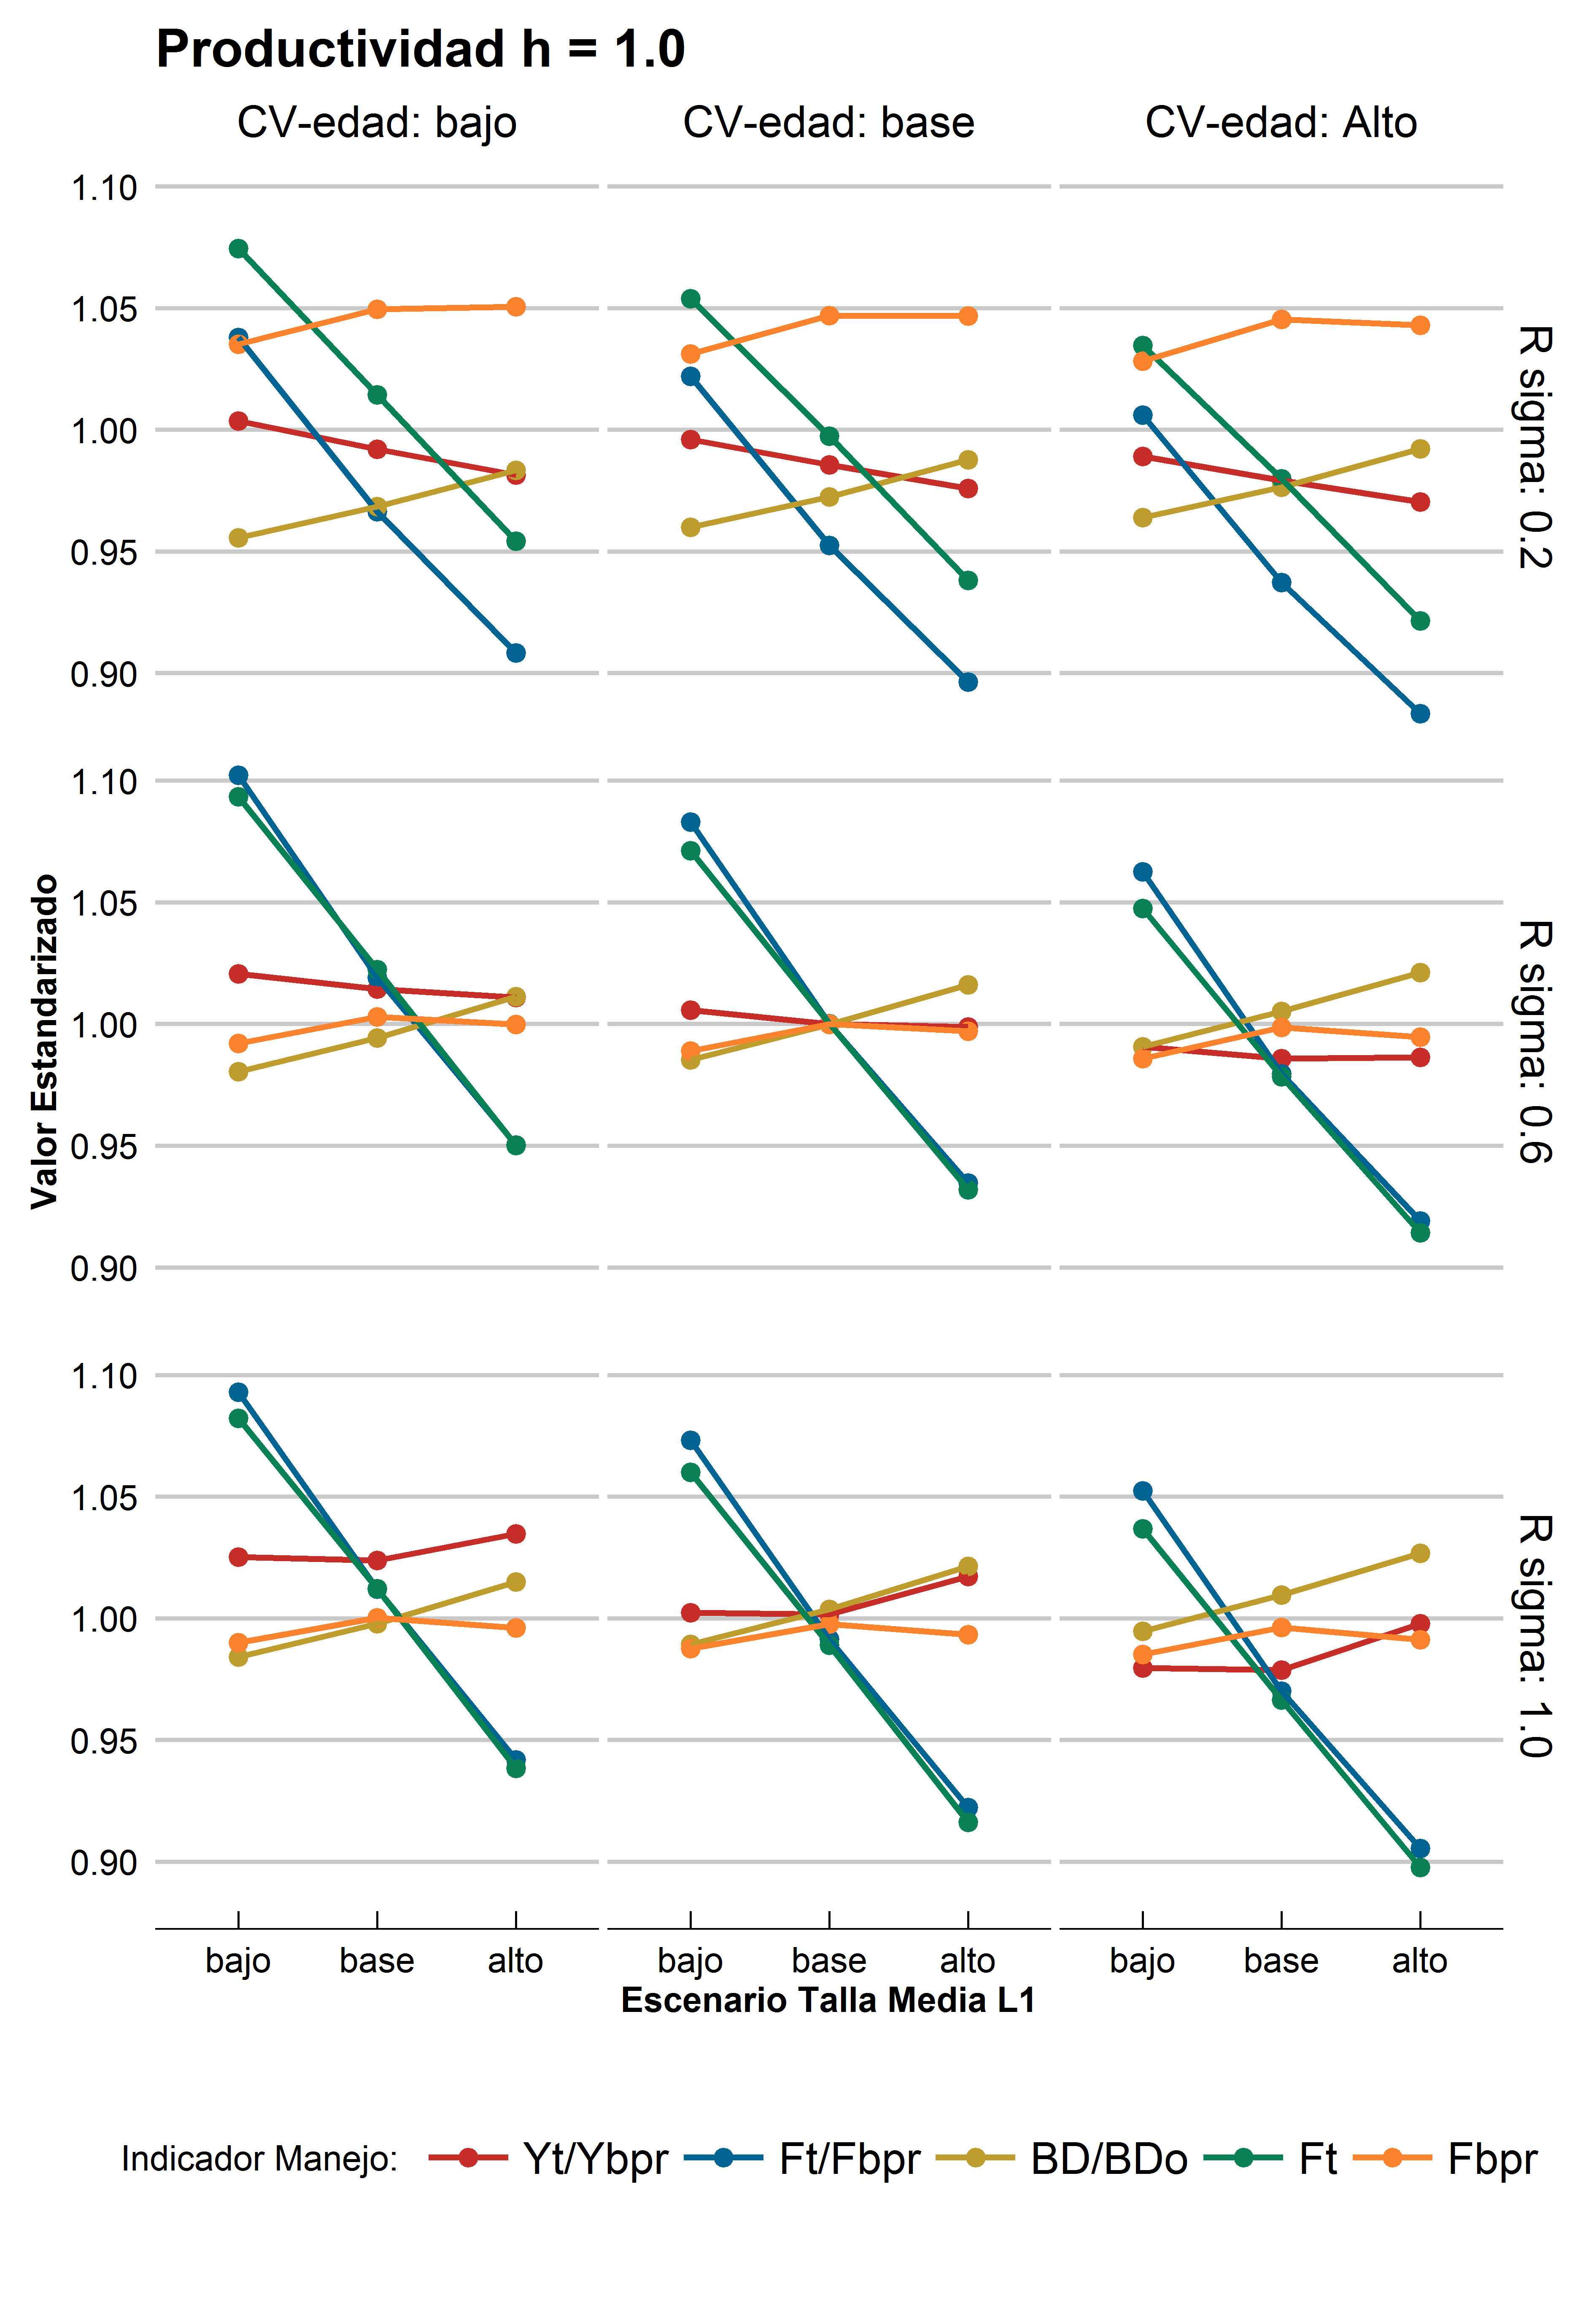
\includegraphics[width=0.70\columnwidth]{figures/steepness-10-var.png}
  \end{center}
\caption{Management advice indicators for scenario with productivity h=1.0. Contained the results of nine (9) scenarios of growth, (x-axis: mean length at-age L1) low (-10\%), Base, high (+10\%). Each column correspond to scenario of VLA, low (-10\%), Base, high (+10\%). Each row correspond to a recruitment variance value.}
\label{figure1}
\end{figure}


\begin{figure}[hbtp]
	\begin{center}
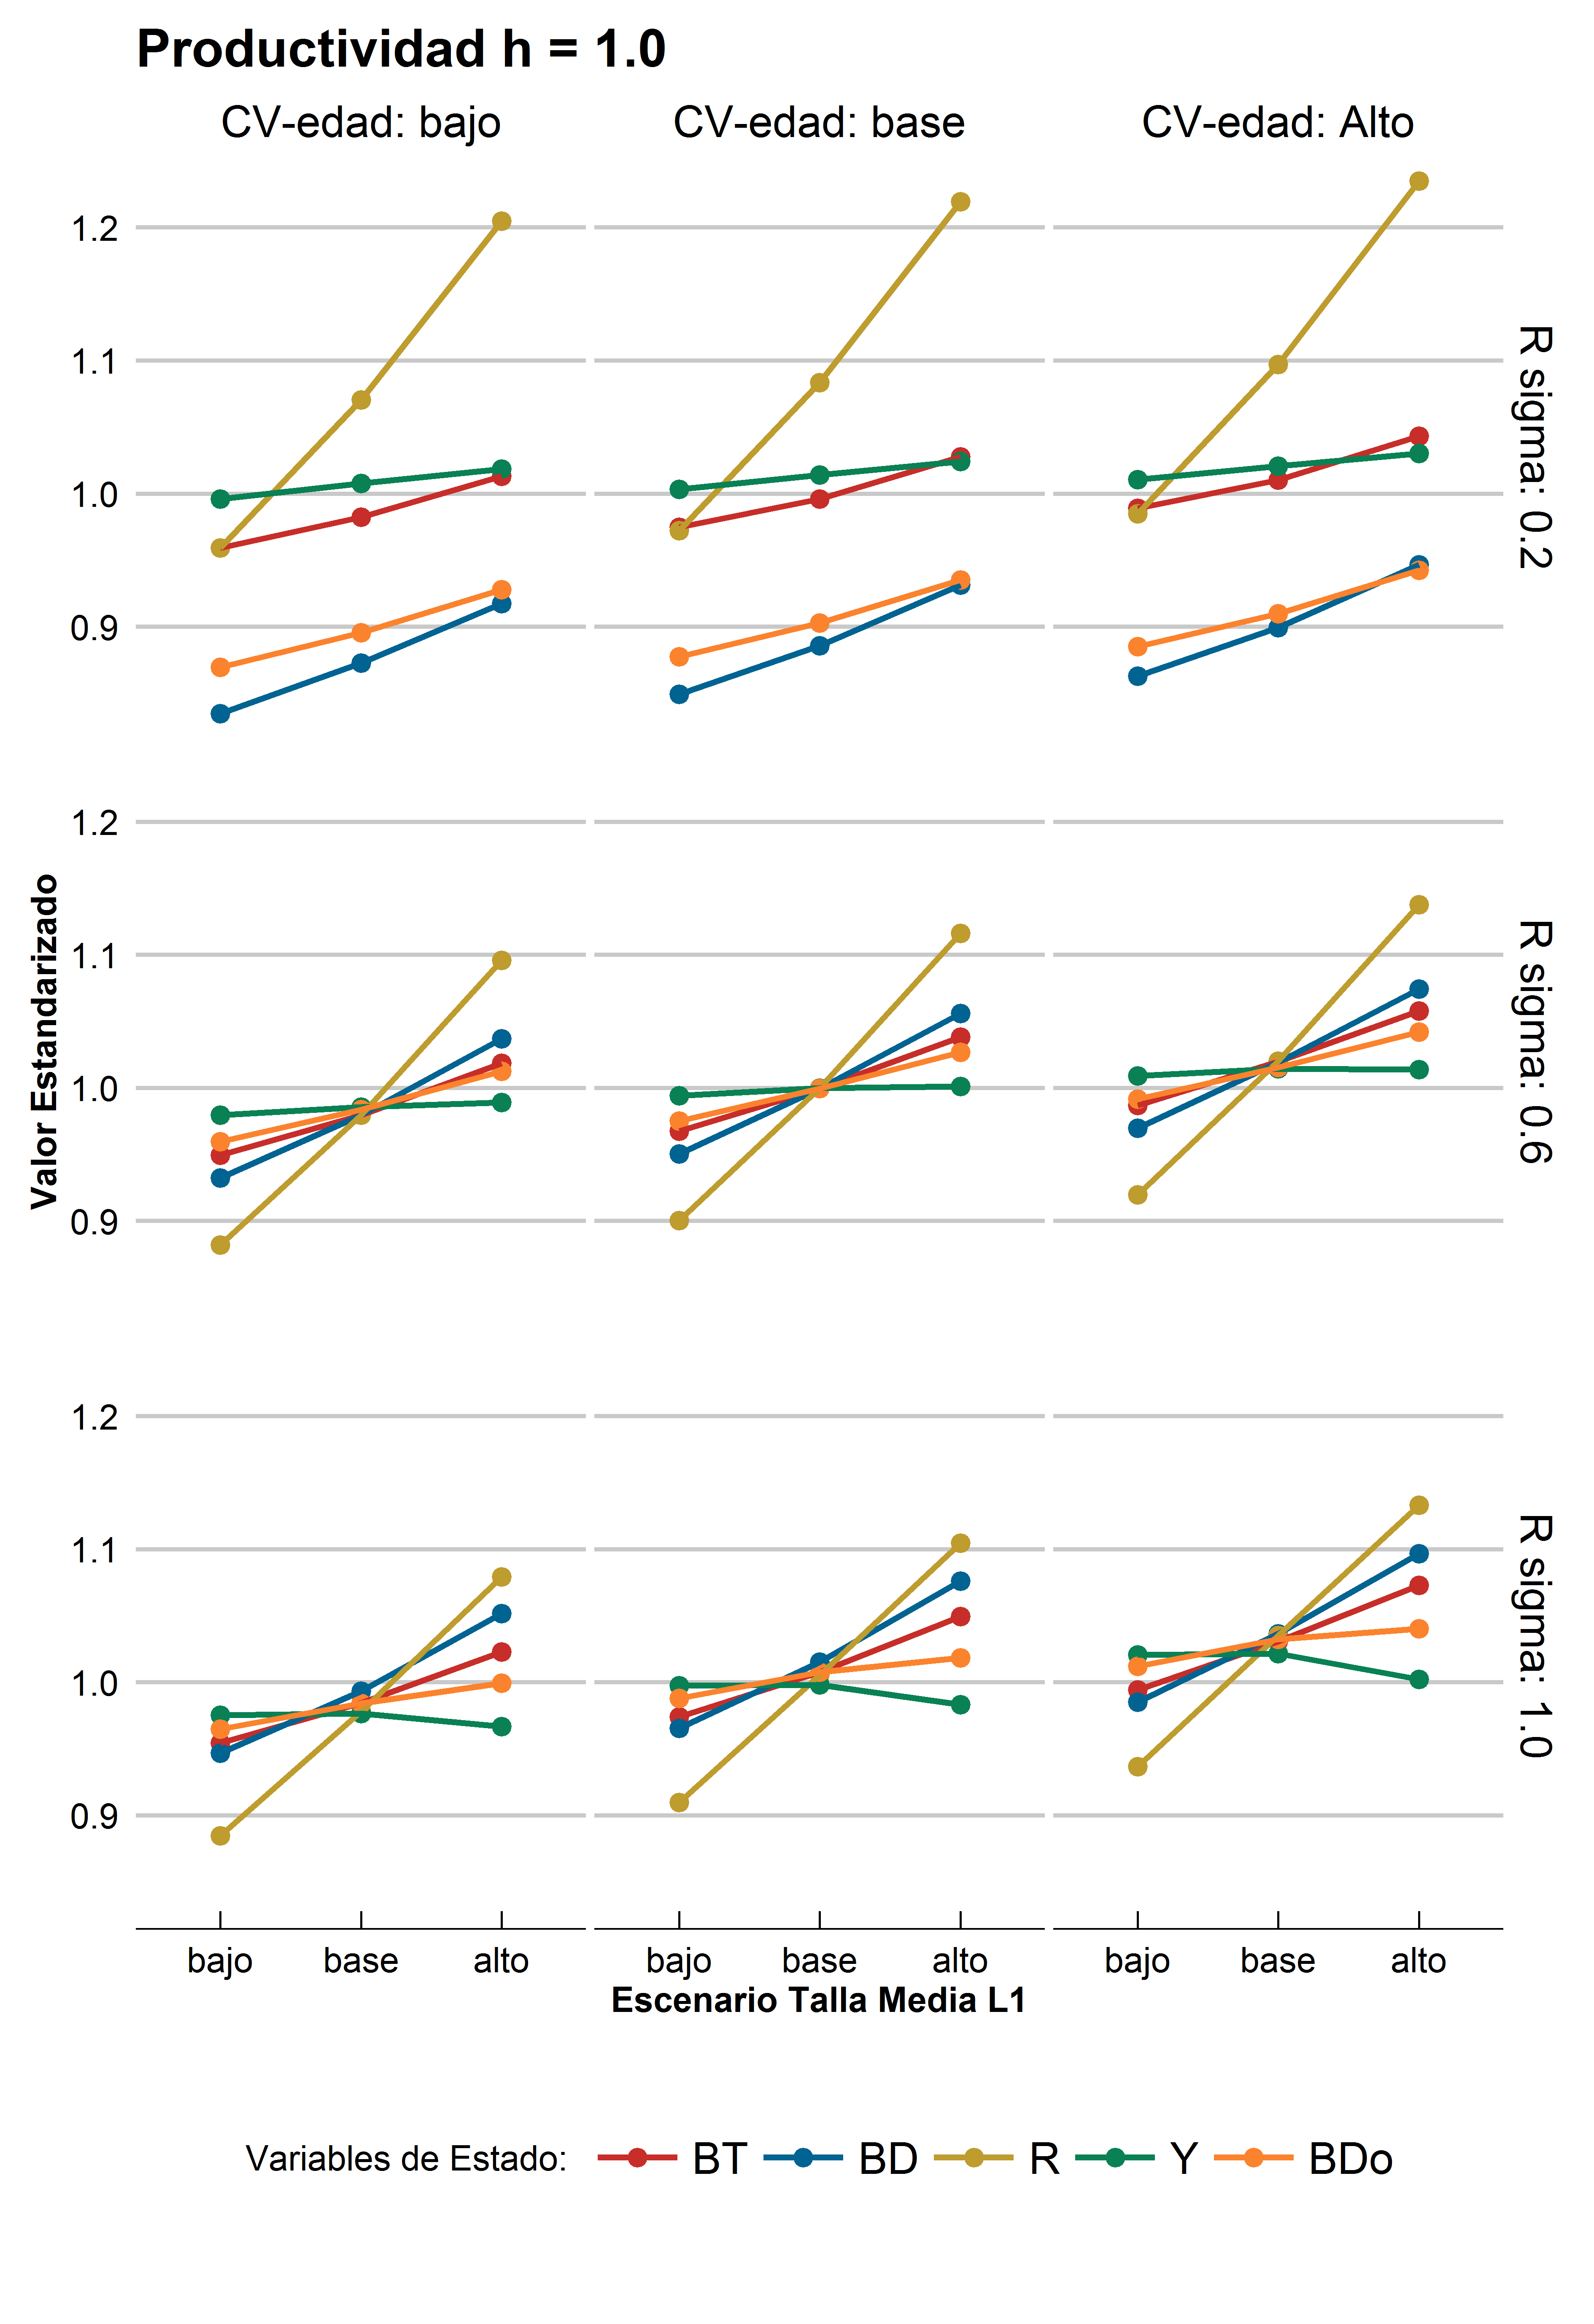
\includegraphics[width=0.70\columnwidth]{figures/steepness-10-estado.png}
  \end{center}
\caption{Stock assessment variables for scenario with productivity h=1.0. Contained the results of nine (9) scenarios of growth, (x-axis: mean length at-age L1) low (-10\%), Base, high (+10\%). Each column correspond to scenario of VLA, low (-10\%), Base, high (+10\%). Each row correspond to a recruitment variance value. Dashed black rectangle indicates the Base Case and should be equal to h=1. TODO---include rectangle}
\label{figure1}
\end{figure}


\begin{figure}[hbtp]
	\begin{center}
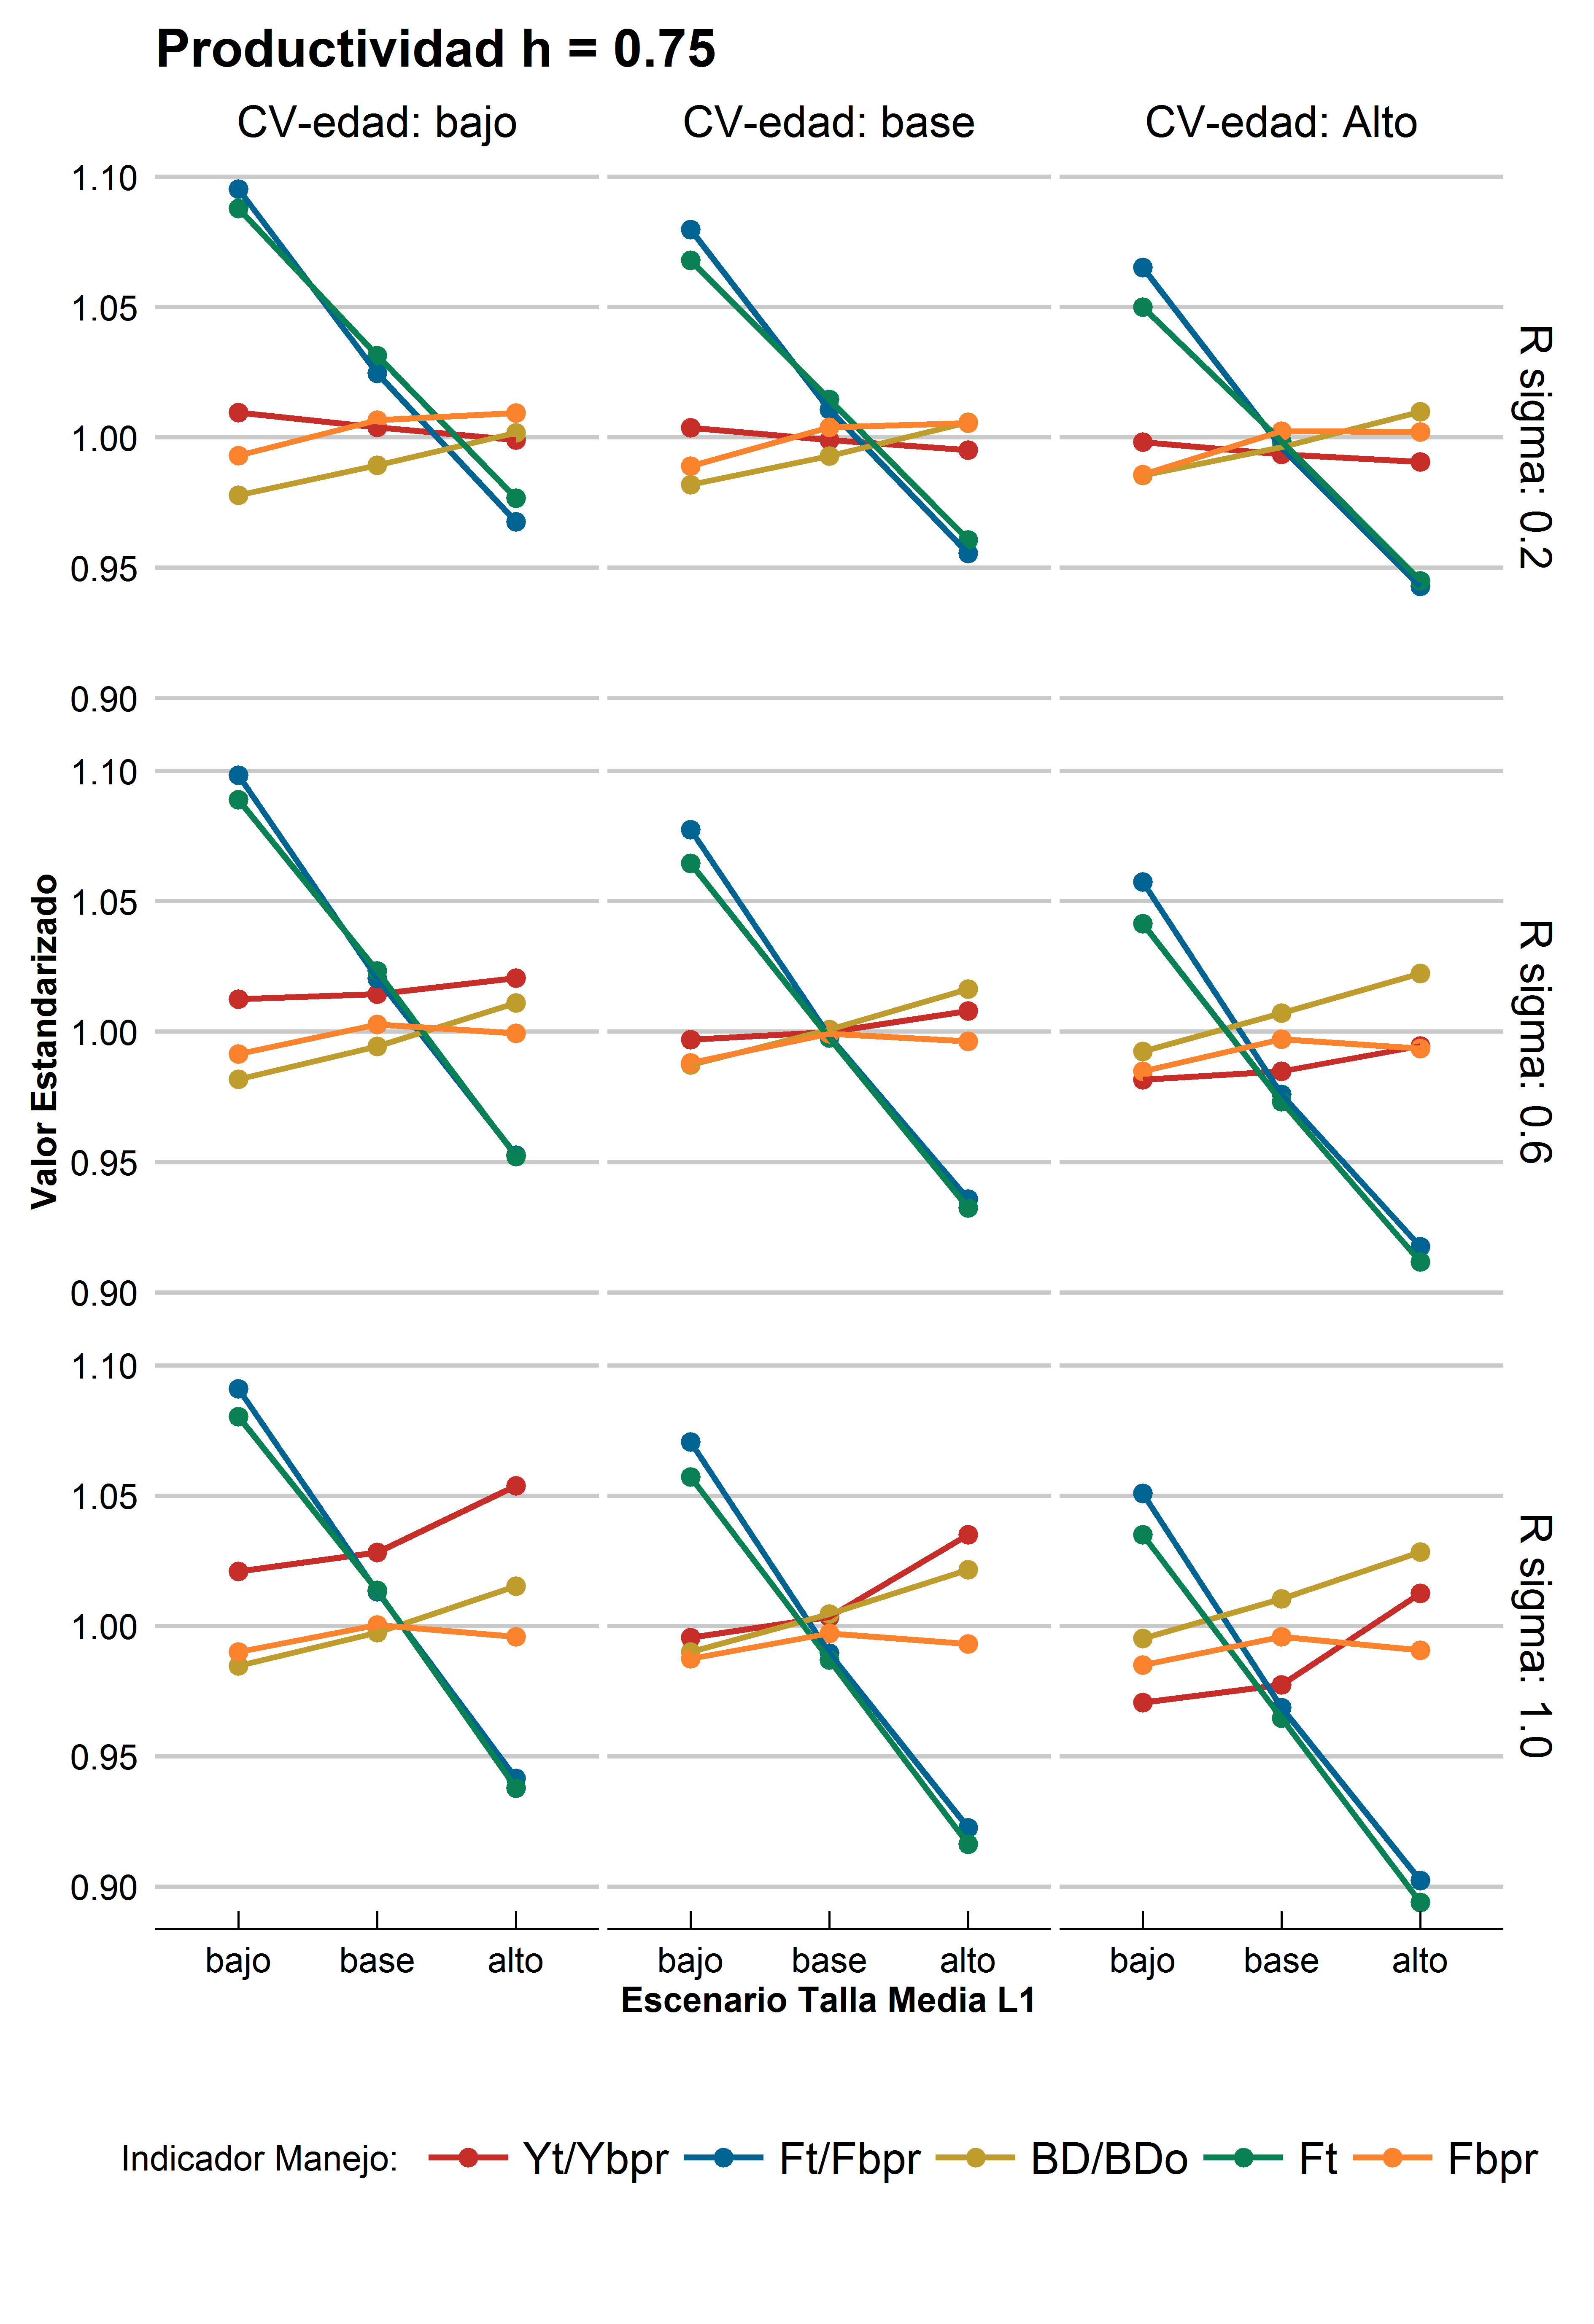
\includegraphics[width=0.70\columnwidth]{figures/steepness-75-var.png}
  \end{center}
\caption{Management advice indicators for scenario with productivity h=0.75. Contained the results of nine (9) scenarios of growth, (x-axis: mean length at-age L1) low (-10\%), Base, high (+10\%). Each column correspond to scenario of VLA, low (-10\%), Base, high (+10\%). Each row correspond to a recruitment variance value.}
\label{figure1}
\end{figure}


\begin{figure}[hbtp]
	\begin{center}
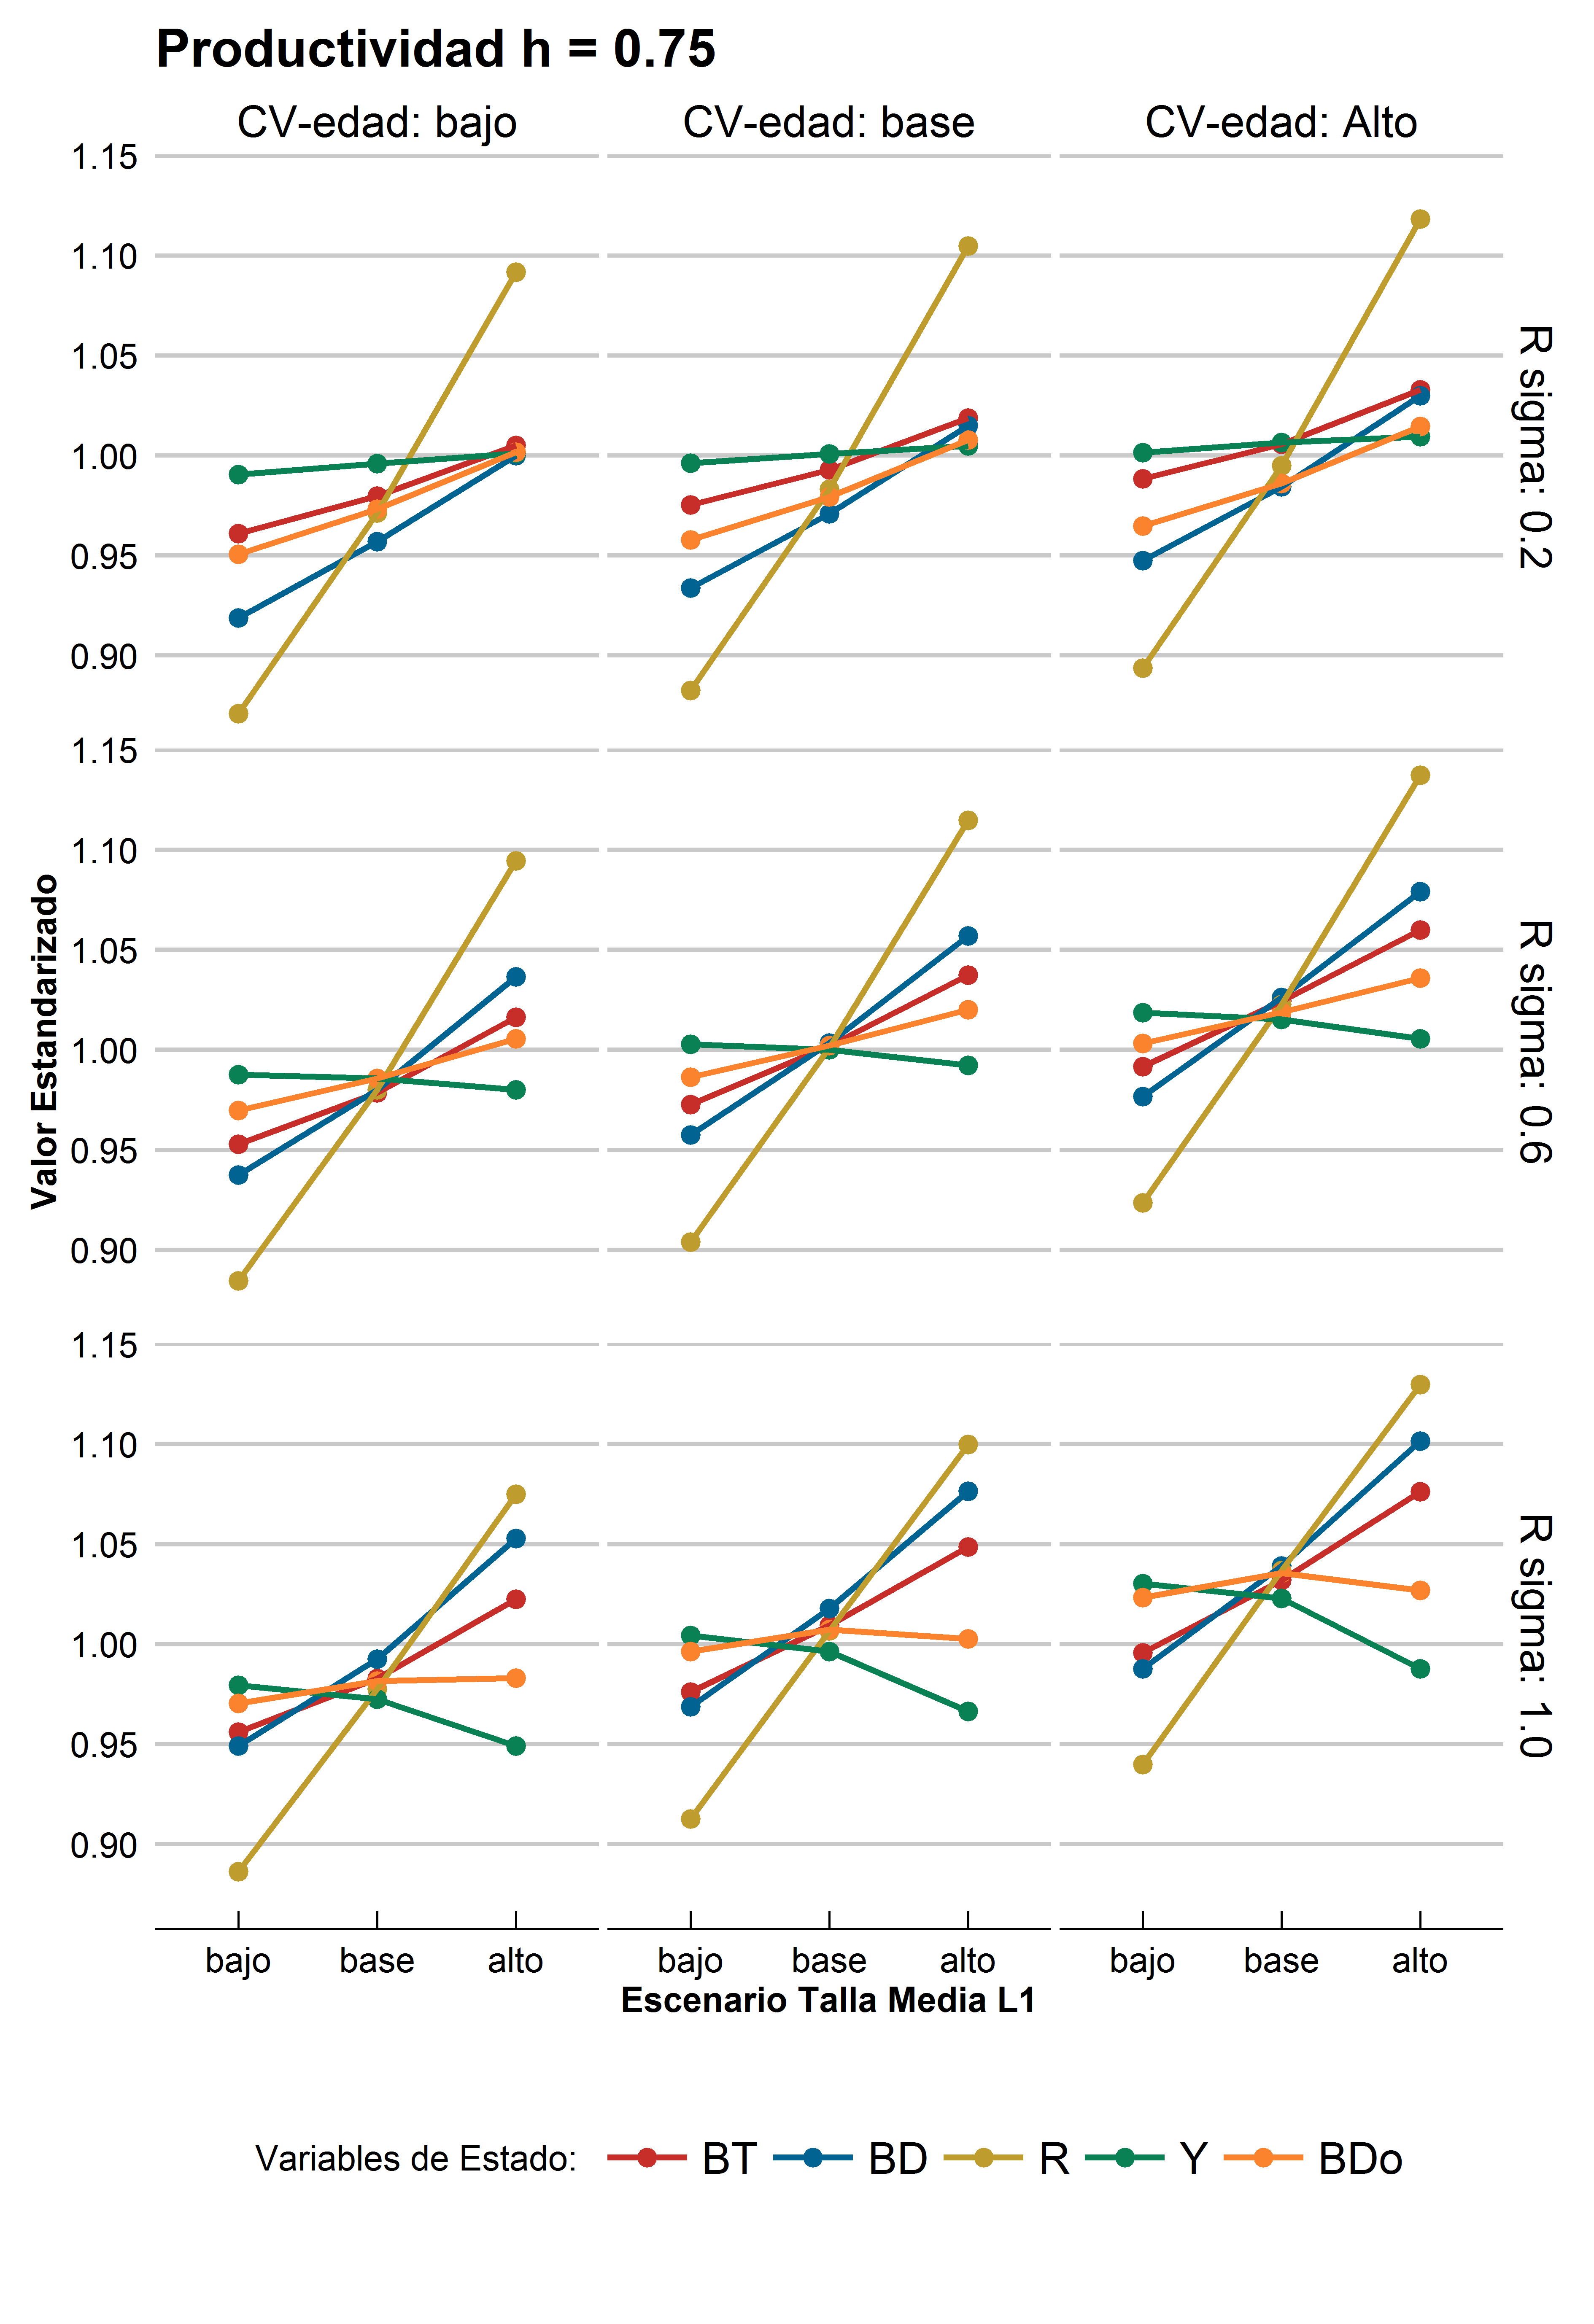
\includegraphics[width=0.70\columnwidth]{figures/steepness-75-estado.png}
  \end{center}
\caption{Stock assessment variables for scenario with productivity h=0.75. Contained the results of nine (9) scenarios of growth, (x-axis: mean length at-age L1) low (-10\%), Base, high (+10\%). Each column correspond to scenario of VLA, low (-10\%), Base, high (+10\%). Each row correspond to a recruitment variance value. Dashed black rectangle indicates the Base Case and should be equal to h=1. TODO---include rectangle}
\label{figure1}
\end{figure}

\end{document}
